%%%%%%%%%%%%%%%%%%%%%%%%%%%%%%%%%%%%%%%%%%%%%%%%%
%%             SqueakBot Pas à Pas             %%
%%                                             %%
%%         Planète Sciences 2009-2010          %%
%%%%%%%%%%%%%%%%%%%%%%%%%%%%%%%%%%%%%%%%%%%%%%%%%

%% Authors: Séverin Lemaignan


%\documentclass[a4paper,12pt,twoside]{article}
\documentclass[a4paper,12pt]{book}

\usepackage{graphicx}

\usepackage{xcolor}

\usepackage{ifthen}

\usepackage[utf8]{inputenc}
\usepackage{listings}

\usepackage{fancyhdr} %headers and footers

\usepackage{url}
\usepackage{hyperref}
\usepackage{sectsty}

\usepackage{enumerate}

% Fixme notes
\usepackage[draft,footnote,marginclue]{fixme}

\usepackage[toc]{glossaries}

\usepackage[french]{babel}

%%%%%%%%%%%%%%%%%%%%%%%%%%%%%%%%%%%%%%%%%%%%%%%%%%%%%%%%%%%%%%%%%%%%%%%%%%%%%%%
%%                           Glossary                                        %%
%%%%%%%%%%%%%%%%%%%%%%%%%%%%%%%%%%%%%%%%%%%%%%%%%%%%%%%%%%%%%%%%%%%%%%%%%%%%%%%
\makeglossaries
%Pour re-générer le glossaire : makeindex squeakbot_pas_a_pas.glo -s squeakbot_pas_a_pas.ist -t squeakbot_pas_a_pas.glg -o squeakbot_pas_a_pas.gls

\newglossaryentry{halo}
		{name={halo}, 
		description={C'est l'ensemble des icônes qui entourent un objet quand on fait un \cd dessus}}
\newglossaryentry{script}
		{name={script}, 
		description={Les scripts sont les programmes associés à chaque objet}}
\newglossaryentry{visualisateur}
		{name={visualisateur}, 
		description={Le visualisateur est la zone, spécifique à chaque objet, qui contient toutes les briques permettant la programmation. On l'affiche grâce à \icon[\og \oe il \fg]{oeil} du halo de l'objet}}
\newglossaryentry{cap}
		{name={cap}, 
		description={Le cap d'un objet est son orientation absolue (en degrés) : un cap de 0 équivaut à une orientation vers le haut de l'écran. Pour modifier le cap, il faut faire tourner un peu l'objet avec \icon{pivoter}, puis cliquer sur la flèche verte \important{en maintenant la touche \textit{Majuscule} appuyée}}}
\newglossaryentry{parametre}
		{name={paramètre}, 
		description={Un paramètre d'une fonction est une option que l'on passe à la fonction et que l'on peut modifier.}}
\newglossaryentry{monde}
		{name={Monde}, 
		description={Le \og monde \fg est l'ensemble du bureau de \appName. C'est un objet similaire aux autres~: on peut afficher son halo, son visualisateur, lui associer des scripts...}}
%%%%%%%%%%%%%%%%%%%%%%%%%%%%%%%%%%%%%%%%%%%%%%%%%%%%%%%%%%%%%%%%%%%%%%%%%%%%%%%

\def\appName{SqueakBot}
%\def\appName{EToys}

%A remplacer par des images ?
\def\cd{clic droit~}
\def\cm{clic du milieu~}
\def\cg{clic gauche~}

\newcommand{\capture}[1]
{
\begin{center}
	\includegraphics[scale=0.5]{#1}
\end{center}
}

\newcommand{\brique}[1]
{
\fcolorbox[RGB]{200,192,144}{200,248,200}{\textbf{#1}}
}

%Commande pour la mise en forme du code, comme les noms de scripts
\newcommand{\code}[1]
{
\texttt{#1}
}

\newcommand{\important}[1]
{
\textbf{#1}
}

\newcommand{\motcle}[2]
{
\important{\gls{#1}}
}


\newcommand{\inserticon}[1]
{
\includegraphics[scale=0.5]{icons/#1.png}
}
%Cette macro peut être utilisée pour facilement insérer les icônes de Squeak dans
%le document.
% \icon{nom_de_l_icone_sans_extension} affiche juste l'icône, inline ;
% \icon[nom]{nom_de_l_icone_sans_extension} affiche "l'icône [image] nom"
\newcommand{\icon}[2][]
{
\ifthenelse {\equal{#1} {}} {\inserticon{#2}} {l'icône \inserticon{#2} \important{#1}}
}

% A encadrer, avec un p'tit logo
\newcommand{\afaire}[1]
{
#1
}

%Met par defaut la taille en scriptsize et la font en sans serif pour les notes dans la marge
\let\myMargin\marginpar
\renewcommand{\marginpar}[1]{\myMargin{{\scriptsize \sffamily #1}}}


\graphicspath{{captures/}}

%################# En-tête et pieds de page avec fancyhdr
\headheight=14.85pt
%pour récupérer les noms de section en minuscule
\renewcommand{\chaptermark}[1]{\markboth{\sffamily #1}{}}
\renewcommand{\sectionmark}[1]{\markright{\sffamily #1}}

\fancyhf{}
\fancyhead[RO]{\bfseries\rightmark}
\fancyhead[LE]{\bfseries\leftmark}
\fancyfoot[LE,RO]{\bfseries\thepage}
\renewcommand{\headrulewidth}{0.5pt}
\addtolength{\headheight}{0.5pt}
\renewcommand{\footrulewidth}{0pt}
\fancypagestyle{plain}{\fancyhead{}\renewcommand{\headrulewidth}{0pt}}

%%%%%%%%%%%%%%%%%%%%%%%%%%%%%%%%%%%%%%%%%%%%%%%%%%%%%%%%%%%%%%%%%%%%%%%%%%%%%%%%%%%%%%%%%%%%%%%%%%%%%%%
%%%%%%%%%%%%%%%%%%%%%%%%%%%%%%%%%%%%%%%%%%%%%%%%%%%%%%%%%%%%%%%%%%%%%%%%%%%%%%%%%%%%%%%%%%%%%%%%%%%%%%%

%%%%%%%%%%%%%%%%%%%%%%%%%%%%%%%%%%%%%%%%%%%%%%%%%
%%        LÀÀÀÀÀÀÀÀÀÀÀÀÀÀÀÀÀÀ !!               %%
%%                                             %%
%% Juste en-dessous, ça définit la première    %%
%% page. Ensuite, c'est le "vif" du sujet. Tu  %%
%% va voir, ce n'est pas très compliqué !      %%
%%%%%%%%%%%%%%%%%%%%%%%%%%%%%%%%%%%%%%%%%%%%%%%%%


\title{
	
\includegraphics[width=3cm]{national.png}\\
	\vfill
%	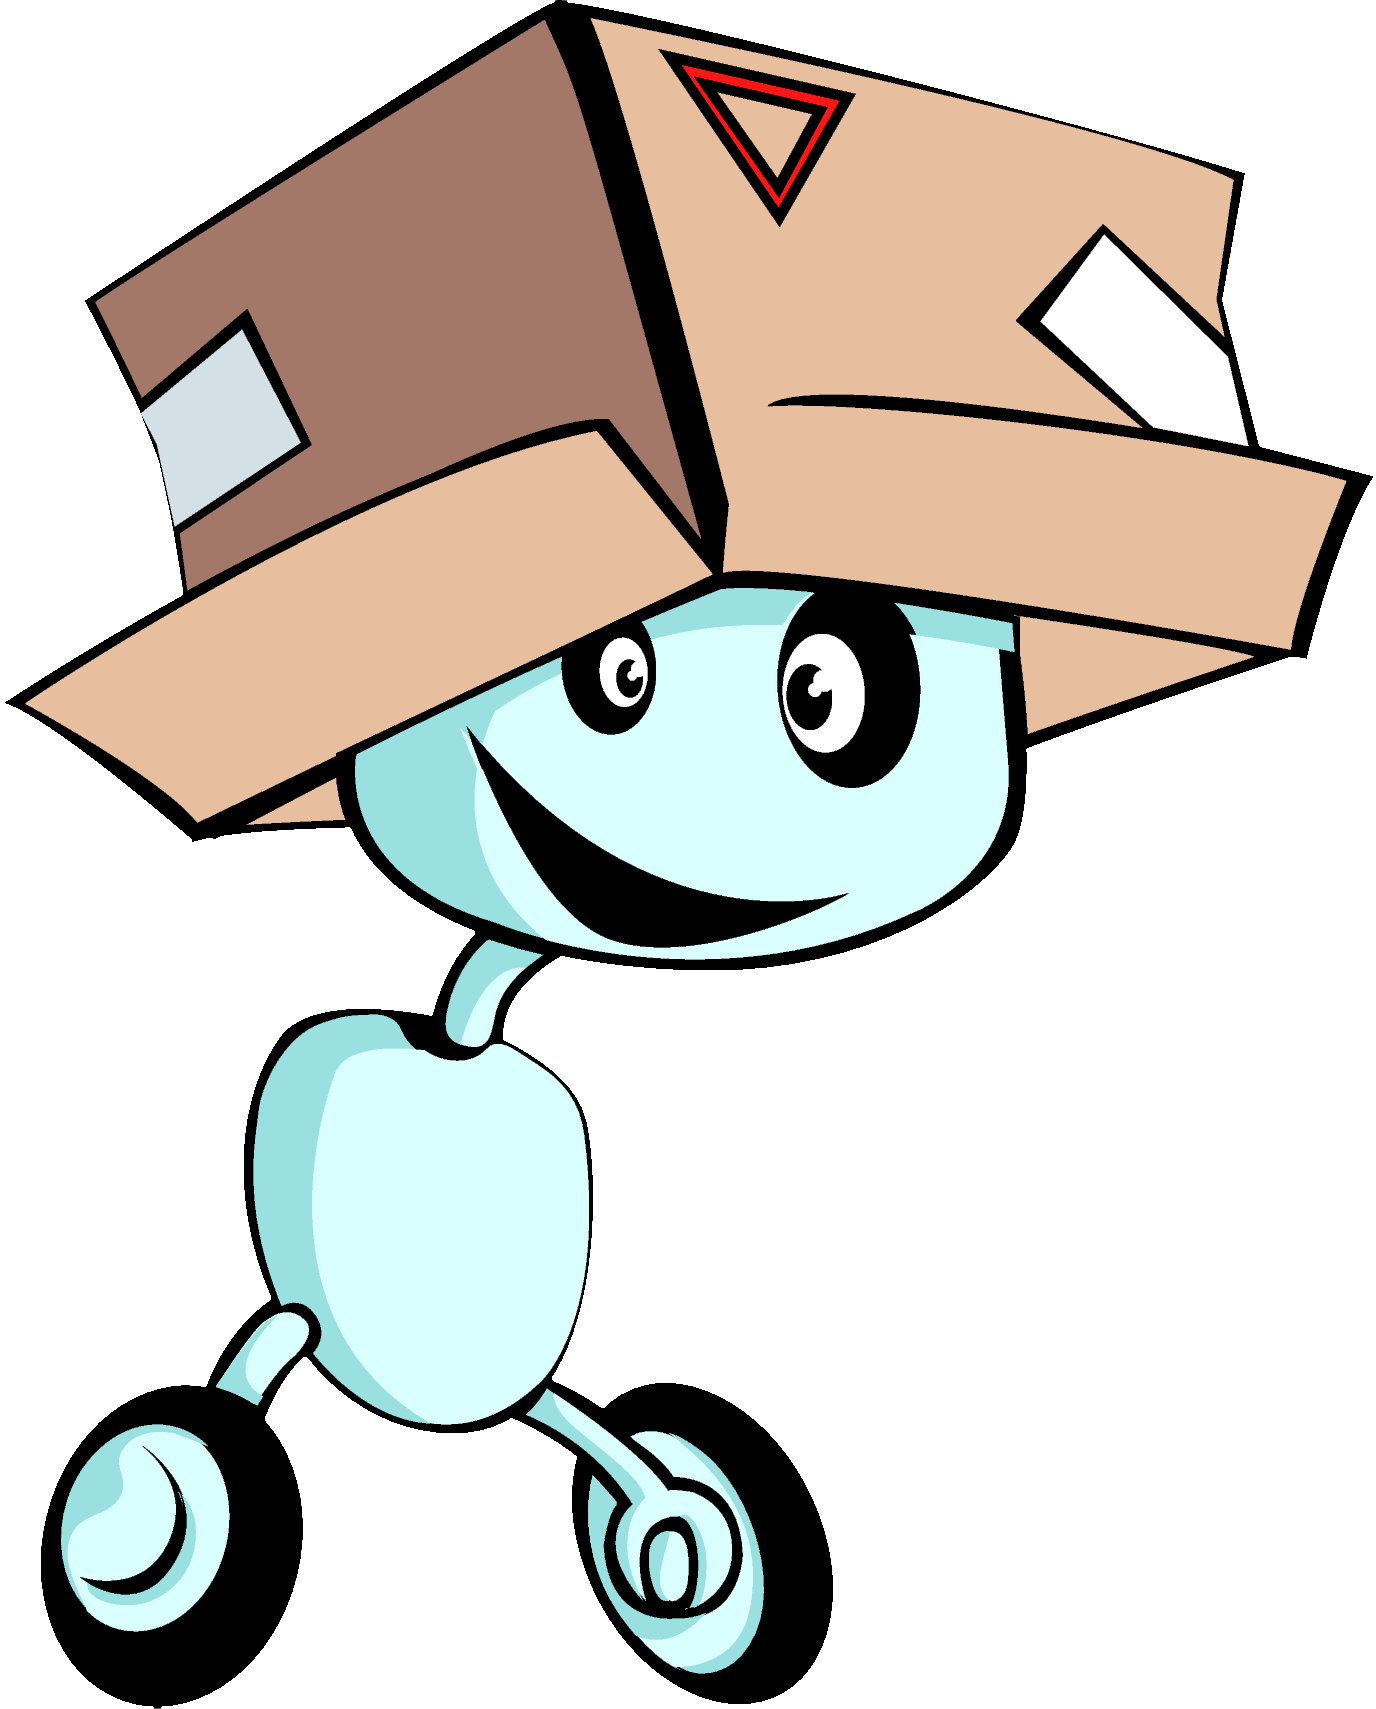
\includegraphics[width=5cm]{minibot.png}
	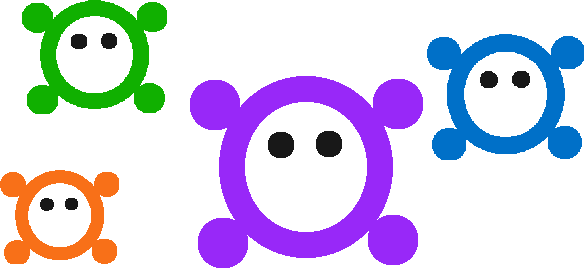
\includegraphics[width=5cm]{bestioles.png}\\
	\vspace{3em}
	\LARGE{\textbf{\appName~et les bestioles}}\\[1cm]
	\large{Une aventure pour découvrir pas à pas \appName}\\[1cm]
	\vfill
}

\author{
Planète Sciences
}

%%%%%%%%%%%%%%%%%%%%%%%%%%%%%%%%%%%%%%%%%%%%%%%%%%%%%%%%%%%%%%%%%%%%%%%%%%%%%%%%%%%%%%%%%%%%%%%%%%%%%%%
%%%%%%%%%%%%%%%%%%%%%%%%%%%%%%%%%%%%%%%%%%%%%%%%%%%%%%%%%%%%%%%%%%%%%%%%%%%%%%%%%%%%%%%%%%%%%%%%%%%%%%%
\begin{document}

\sffamily
\allsectionsfont{\sffamily}

\maketitle

\tableofcontents

%%%%%%%%%%%%%%%%%%%%%%%%%%%%%%%%%%%%%%%%%%%%%%%%%%%%%%%%%%%%%%%%%%%%%%%%%%%%%%%%%%%%%%%%%%%%%%%%%%%%%%%
%%%%%%%%%%%%%%%%%%%%%%%%%%%%%%%%%%%%%%%%%%%%%%%%%%%%%%%%%%%%%%%%%%%%%%%%%%%%%%%%%%%%%%%%%%%%%%%%%%%%%%%

\clearpage
~
\vfill
\begin{center}
    \LARGE{\textbf{Le prologue}}
\end{center}

\vspace{3em}

L'une des forces et, en réalité, la principale raison d'être de \appName, c'est qu'il permet aux enfants, jeunes et moins jeunes, d'expérimenter autant qu'ils le souhaitent, sans jamais se demander si ce qu'il font est juste ou faux, bon ou pas bon.

Les pages qui suivent proposent une découverte approfondie de \appName dans le cadre de la réalisation d'un projet relativement complexe, qui devrait permettre à chacun de devenir vraiment à l'aise à l'intérieur de l'interface parfois un peu déroutante de \appName, tout en mesurant l'étendue des possibilités qu'il ouvre.

Cependant ce tutoriel ne devrait sans doute pas être utilisé tel quel pour mener un projet avec les enfants. Il ne s'agit en particulier pas de remettre ce livret dans les mains des enfants et de leur dire \og Amusez-vous bien~! \fg~: à suivre pas à pas le projet, ils passeraient à côté de cet esprit d'expérimentation, ce vent de créativité que nous voulons développer.

Nous ne pouvons donc que vous encourager à vous servir de ce livre comme un outil pour votre propre pratique, comme une référence, comme une source d'idée, et ponctuellement, comme un guide pour les enfants.

Bonne découverte !

\vfill

%%%%%%%%%%%%%%%%%%%%%%%%%%%%%%%%%%%%%%%%%%%%%%%%%%%%%%%%%%%%%%%%%%%%%%%%%%%%%%%%%%%%%%%%%%%%%%%%%%%%%%%
%%%%%%%%%%%%%%%%%%%%%%%%%%%%%%%%%%%%%%%%%%%%%%%%%%%%%%%%%%%%%%%%%%%%%%%%%%%%%%%%%%%%%%%%%%%%%%%%%%%%%%%
\chapter{Bienvenue !}

Bienvenue ! Dans les pages qui suivent, nous allons ensemble, étape par étape, découvrir \appName. C'est une univers un peu déroutant au début, mais c'est un vrai univers~: dans \appName, toutes les histoires peuvent être racontées~! L'objectif, c'est qu'il soit facile de donner vie à toutes les idées qui nous passent par la tête, que ce soit des manchots qui sautent sur le dos d'une baleine, des fleurs qui dansent, ou des bestioles bizarroïdes qui se multiplient.

Des bestioles bizarroïdes qui se multiplient~?

\begin{center}
    
\includegraphics[width=4cm]{bestiole.png}
\end{center}

Des bestioles comme ça, peut-être~?

\fixme{Insérer une capture avec plein de bestioles}

Qui se multiplient comme ça~?

...et pourquoi pas, tiens~! Allez, lançons nous dans ce projet : Faire, en partant de zéro, une petite simulation d'écosystème, avec des bestioles qui naissent, qui se reproduisent, qui se nourrissent et qui meurent. Voyons ce que ça peut donner.

%%%%%%%%%%%%%%%%%%%%%%%%%%%%%%%%%%%%%%%%%%%%%%%%%%%%%%%%%%%%%%%%%%%%%%%%%%%%%%%%%%%%%%%%%%%%%%%%%%%%%%%
%%%%%%%%%%%%%%%%%%%%%%%%%%%%%%%%%%%%%%%%%%%%%%%%%%%%%%%%%%%%%%%%%%%%%%%%%%%%%%%%%%%%%%%%%%%%%%%%%%%%%%%
\chapter{Prendre en main \appName}

\section{Le monde des objets}

Au démarrage de \appName, vous devriez tomber sur quelque chose qui ressemble de près à l'image ci-dessous :

\capture{0.png}

Voici les principales fonctions des différents boutons que l'on voit dans l'interface :

\capture{2.png}

Faisons un \cd sur le robot Minibot :
\capture{1.png}

Toute une série de petites icônes apparaissent. C'est ce qu'on appelle le \motcle{halo}. C'est elles qui vont nous permettre de jouer avec nos objets.

Voici le rôle des principales d'entre elles :

\capture{3.png}

En cliquant (et en restant appuyé) sur\icon[Pivoter]{pivoter}, on peut faire tourner l'objet :

\capture{4.png}

Nous verrons plus tard à quoi servent les autres icônes et comment modifier le cap et le centre de rotation d'un objet.

En attendant, essaie de redimensionner Minibot avec \icon[Redimensioner]{redimensionner}.

Avant de continuer, faisons un peu de place : clique sur les objets qui sont sur le bureau pour les saisir, et glisse le texte et Minibot sur la corbeille. Si tu le souhaites, tu peux les y récupérer plus tard en double-cliquant sur la corbeille.

Voilà, avec ces premiers pas, nous avons vu ce qu'était un objet dans \appName, et nous avons découvert son halo, et les manipulations de base qui lui sont associées. Nous sommes en bonne route vers la programmation, mais avant cela, voyons comment créer nos propres objets en les dessinant.

\section{La palette des artistes}

Dans \appName, la plupart des objets sont créés à partir de dessin. Pas de limite à notre imagination !

Pour démarrer un dessin, il suffit de cliquer sur l'icône de la palette, en haut de l'écran :

\begin{center}
    
\includegraphics[width=3cm]{palette.png}
\end{center}

Ceci ouvre le mode dessin :

\capture{5.png}

Au centre de l'écran apparait une zone blanche : c'est le \important{calque de dessin}. Tout le dessin doit tenir dedans, et s'il est trop petit, on peut le redimensionner comme tous les objets, en faisant un \cd dessus, puis en utilisant \icon{redimensionner}.

L'illustration ci-dessous présente les différentes fonctionalités de la palette de dessin :

\capture{6.png}

\afaire{Avec ça, ça ne devrait pas poser de problèmes pour dessiner une bestiole ! (pense à utiliser les formes géométriques qui sont dans le tiroir en bas à droite).}

\begin{center}
    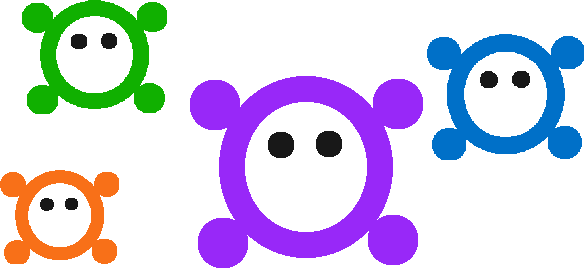
\includegraphics[width=8cm]{bestioles.png}
\end{center}

\afaire{
Une fois notre dessin terminé, nous pouvons cliquer sur \textbf{Fini} pour quitter le mode dessin : ça y est, nous venons de créer un nouvel objet.

Donnons lui un nom en faisant un \cd dessus, puis un \cg sur le mot \texttt{Dessin}. Nous pouvons maintenant taper le nom que nous voulons, suivi de \textit{Entrée}.
}

\capture{7.png}

Nous sommes maintenant prêt pour la programmation !

\section{Notre premier programme}
\label{premier_programme}

Nous avons fait connaissance avec les objets. Si nous essayions maintenant de leur donner vie~? Leur donner vie, ça va être, pour nous, associer à nos objets des \important{programmes} qui vont par exemple les faire bouger ou les modifier.\marginpar{Dans \appName, les programmes sont intimement liés aux objets. Chaque objet a ses propres programmes. C'est pour cela que \important{Smalltalk}, le langage de programmation qui est derrière \appName est appelé \important{langage orienté objet}.}

Le point de départ pour tous les programmes (ou \motcle{script}, comme nous allons les appeler dans \appName), c'est le \motcle{visualisateur} de chaque objet.

Pour ouvrir le visualisateur, il suffit de cliquer sur \icon[\og \oe il \fg]{oeil} du halo de notre objet :

\capture{8bis.png}

Le visualisateur est l'élément d'interface qui à l'air le plus compliqué dans \appName. En fait, son organisation est plutôt simple, mais comme il permet d'accéder à presque toutes les fonctions de programmation des objets, beaucoup de choses sont affichées.

Comme le montre l'illustration ci-dessous, le visualisateur se compose de grandes catégories (dans l'exemple ci-dessous, on voit les catégories \og Briques de base \fg et \og Tests \fg) qui contiennent un certain nombre de briques.

\capture{9.png}

Nous verrons un peu plus tard les différents types de brique. Pour l'instant, essayons de faire notre premier programme, pour faire bouger notre bestiole. Pour cela, faisons un \cg sur la brique \brique{avance de 5}, et glissons cette brique sur le bureau, à côté du dessin de l'objet :

\capture{10bis.png}

Étudions un peu plus en détail la nouvelle fenêtre de script qui vient d'apparaitre :

\capture{11bis.png}

Les scripts peuvent soit être exécuté juste une fois en cliquant sur le point d'exclamation jaune (dans notre cas, notre bestiole va donc avancer de 5 pixels), soit ils peuvent être démarrés pour de bon.

Si tu cliques sur la petite horloge à côté de \textit{normal}, tu démarres le script. Cela veut dire que, tant que tu ne le mettras pas en pause en re-cliquant sur l'horloge, \appName va exécuter en boucle le contenu du script. Essaie donc !

Normalement, la bestiole devrait se mettre à bouger vers le haut : en réalité, elle avance dans la direction de son \motcle{cap}. Nous verrons un peu plus tard ce que signifie le cap, et comment le modifier.

À n'importe quel moment, même quand le programme est en marche, tu peux cliquer sur ton dessin pour le prendre et le déplacer ailleurs sur le bureau. C'est pratique quand ton objet est coincé contre un bord, par exemple.

Essayons maintenant de compléter le script pour que la bestiole tourne en même temps qu'elle avance. Pour cela, prennons la brique \brique{tourne de 5} et déposons-là en-dessous ou au-dessus de la brique \brique{avance de 5}, à l'intérieur du script que nous avons créé.

\capture{12.png}

Si ton script était déjà en marche, tu devrais voir ta bestiole commencer à tourner, sinon, met-le en route.\marginpar{Le chemin que décrit notre objet s'appelle sa \important{trajectoire}. En faisant varier la vitesse et la vitesse de rotation, on change la trajectoire ! Tu as du remarquer que cette trajectoire a d'ailleurs une forme que tu connais bien~: comment s'appelle-t'elle~?}

Comme nous pouvons le voir, les briques \brique{avance de 5} et \brique{tourne de 5} prennent une vitesse comme option (en programmation, on appelle ça un \motcle{parametre}). Essayons de les faire varier !

\capture{13bis.png}

\afaire{Que penses-tu de cette trajectoire~? Comment pourrait-on faire tourner la bestiole dans l'autre sens~?}

\section{Voir les trajectoires}
\label{traces}
Pour mieux voir la trajectoire de notre bestiole, nous allons lui demander de laisser une trace de son passage.

Pour cela, ouvre la catégorie \textit{Traces}, en cliquant sur le titre d'une des catégories déjà affichées du visualisateur (tu devrais avoir \textit{Scripts}, \textit{Briques de bases} et \textit{Tests}), puis en sélectionnant \textit{Traces}.

\capture{14.png}

Dans le panneau de la catégorie trace, choisis une couleur de trace qui te plait, augmente un peu la largeur de la trace, puis change la brique \brique{laisse trace} pour la mettre à \textit{vrai} (clique sur la flêche du bas ou du haut, à côté de \textit{faux}).

\capture{15.png}

Redémarre ton script si besoin.

\capture{16.png}

Cette fois-ci plus de doute, notre bestiole parcourt un cercle !

Tu peux effacer les traces en cliquant sur le \icon{exclamation} point d'exclamation devant la brique \brique{efface traces}, et recommencer, en changeant la vitesse de ta bestiole. Pour arrêter de laisser des traces, il suffit de remettre à \textit{faux} la brique \brique{laisse trace}.

\section{Un grain de folie !}

...les bestioles, en général, n'ont pas une belle trajectoire circulaire comme cela~: essayons de mettre un peu de folie là-dedans !

Pour cela, nous allons utiliser un peu de ...\important{hasard}.

Si ce n'est pas fait, met ton script en pause en cliquant sur \icon{horlogestop} l'horloge, puis clique sur \icon[Boite à fonctions]{boiteaoutils} dans la fenêtre du script.

\capture{17.png}

Sélectionnons la brique \brique{hasard}, et glissons-là \important{à la place} de la vitesse que nous avions auparavant. Faisons de même pour la vitesse de rotation de la brique \brique{tourne de} :

\capture{18.png}

Démarrons le script ! Quelque chose à l'air de clocher : notre bestiole tourne sur elle-même, sans vraiment avancer !

\afaire{Une idée ?}

Logique ! la brique \brique{hasard} nous renvoie une valeur au hasard entre 0 et la valeur qu'on lui donne en paramètre (dans l'exemple au-dessus, une valeur entre 0 et 10 pour la vitesse, et entre 0 et 15 pour la vitesse de rotation).

Ça veut dire que la bestiole tourne toujours dans le même sens, vers la droite.

\afaire{Comment faire pour qu'elle tourne parfois à droite, parfois à gauche, pour avoir ainsi une trajectoire qui ait l'air un peu plus hésistante ?}

Si par exemple, on veut que la bestiole tourne de -10 à +10, la solution la plus simple consiste à tirer au sort un nombre entre 0 et 20, et à soustraire 10. Pour faire cela, tu peux utiliser la flèche verte au bout de la ligne de \brique{tourne de} : elle permet d'ajouter des opérations.

\capture{19.png}

Cette fois-ci, nous avons une vraie trajectoire de bestiole qui ne sait pas trop où elle va !

Voilà, nous savons maintenant comment créer un petit programme ! Avant de passer à la suite, une petite astuce : démarre ton script, et pendant que la bestiole bouge, affiche son halo en faisant un \cd dessus. Clique maintenant sur \icon[Dupliquer]{dupliquer} : hop ! tu viens de faire une copie de ta bestiole.

\capture{20.png}

%%%%%%%%%%%%%%%%%%%%%%%%%%%%%%%%%%%%%%%%%%%%%%%%%%%%%%%%%%%%%%%%%%%%%%%%%%%%%%%%%%%%%%%%%%%%%%%%%%%%%%%
%%%%%%%%%%%%%%%%%%%%%%%%%%%%%%%%%%%%%%%%%%%%%%%%%%%%%%%%%%%%%%%%%%%%%%%%%%%%%%%%%%%%%%%%%%%%%%%%%%%%%%%
\chapter{La danse des scripts}

\section{Jouons avec les briques}

Pour continuer, allons explorer quelques unes des catégories de briques disponibles dans le visualisateur. Au chapitre \ref{premier_programme}, nous avions vu comment était organisé le visualisateur. Regardons maintenant de plus près certaines des catégories existantes.

\marginpar{Les tests sont au c\oe ur de tous les programmes informatiques. C'est ce qu'on appelle une \important{Structure de contrôle}}.

Commencons par la catégorie \important{Tests} qui doit déjà être affichée à l'écran (sinon, on peut masquer les autres panneaux avec \icon[Minimiser]{minimiser})~:

\capture{cat_tests.png}

La première brique, \brique{Si Oui Non}, est une pièce essentielle pour construire les programmes. C'est elle qui permet d'ajouter un test. Les autres briques de cette catégories sont les différents tests que nous avons à disposition.


\afaire{

Tentons tout de suite d'utiliser cette brique. Glissons-la dans le script de notre bestiole, en dessous des autres briques, puis ajoutons le test \brique{touche la couleur} en le faisant glisser devant le \brique{Si} :

\capture{21.png}

Le test \brique{touche la couleur} est \code{Vrai} lorsque une certaine couleur de notre objet (pour l'instant, le rouge, comme l'indique le premier petit carré dans la brique de test) touche une autre couleur (pour l'instant, rouge aussi : c'est la couleur du deuxième carré).

Changons la couleur de notre objet qui doit déclencher le test en cliquant sur le premier carré rouge, puis, à l'aide de la pipette qui apparait, en cliquant sur la couleur que nous voulons :

\capture{22bis.png}

Choississons de la même manière comme couleur à détecter la couleur d'une des traces déjà à l'écran.

Maintenant, nous voudrions que notre bestiole s'arrête dès qu'elle touche cette trace. Comment faire ? Il suffit de \important{déplacer} les briques \brique{avance de} et \brique{tourne de} qui sont au-dessus de notre script \important{à l'intérieur} du test, et plus précisement, en face du \brique{Non}. Ainsi, notre bestiole n'avancera et ne tournera \important{que si elle ne touche pas} la couleur de la trace :

\capture{23.png}

Sur l'exemple ci-dessus, le script est en marche, mais la bestiole n'avance pas car elle touche la trace rouge.

}

La catégorie \important{Tests} contient cinq autres tests. Nous en utiliserons certains un peu plus tard. Si vous laissez la souris quelques instants sur chacun d'eux, une bulle d'aide apparait, qui donne un bref descriptif de ce que fait le test.

Passons à la catégorie \important{Divers} qui contient deux briques très utiles, les briques \brique{Montrer} et \brique{Cacher}.

\capture{cat_divers.png}

\afaire{
Modifions notre programme précédent pour faire disparaitre notre bestiole quand elle touche une trace :

\capture{24.png}

\marginpar{N'oubliez pas~! on peut toujours exécuter une action (ou un script) une fois en cliquant sur le \icon{exclamation} point d'exclamation placé devant}
En exécutant le programme, notre bestiole va disparaitre dès qu'elle touche la couleur détectée ...mais si vous affichez toujours la trace de votre bestiole, vous devriez voir la trace repartir ! en effet, vu que notre objet est invisible, les couleurs ne se touchent plus, notre test devient \code{Faux}, et la bestiole repart ! Nous allons voir tout de suite comment améliorer cela.

En attendant, nous pouvons faire réapparaitre la bestiole en cliquant une fois sur le \icon{exclamation} point d'exclamation placé devant la brique \brique{Montrer} dans le visualisateur.
}

\section{Actions, scripts, paramètres...}

Comment faire pour que la bestiole s'arrête, même quand elle est invisible ? Une solution est tout simplement ...d'arrêter le script ! Normalement un script est démarré et arrêté en cliquant sur la \icon{horlogestop} petite horloge. Mais on peut aussi programmer une mise en route ou un arrêt. Les briques pour cela sont dans la catégorie \important{Contrôle des scripts} :

\capture{cat_controle_scripts.png}

\afaire{
Renommons d'abord notre script afin de lui donner un nom clair, par exemple \code{MouvementBestiole}. Pour cela, il faut cliquer sur le nom du script, et entrer le nouveau nom :
\capture{25.png}

Ensuite, si nous ajoutons au script de la bestiole la brique \brique{arrête} en face du \brique{Oui}, et que nous sélectionnons le script \code{mouvement bestiole}, nous devrions voir notre bestiole disparaitre et, cette fois, s'arrêter sur la couleur.

\capture{26.png}
}

Une utilisation bien pratique du contrôle des scripts, c'est de pouvoir faire un bouton d'arrêt d'urgence et de remise à zéro : il s'agit d'ajouter un bouton qui, quand on clique dessus, arrête tous les scripts et remet les objets dans leur état initial.

\afaire {
Pour cela, nous allons commencer par créer un bouton. Pour ce faire, il faut ouvrir le menu \important{Accessoires}, puis cliquer sur le bouton :

\capture{31.png}

\marginpar{On ne peut pas déplacer le bouton simplement en cliquant dessus comme les autres objets. Pour le déplacer, utilisez \icon[Attraper]{attraper} dans le halo du bouton.}
Renommons-le \code{raz} (remise à zéro), et, dans le halo, cliquons sur \icon[Menu]{menu} pour afficher le menu du bouton. L'option \code{Modifier l'étiquette} va nous permettre de changer l'étiquette du bouton pour quelque chose comme \og Remise à zéro \fg.

\capture{32.png}

En cliquant sur l'icône verte, on peut afficher un script qui se déclenchera lorsqu'on appuie sur le bouton :

\capture{33.png}

Ce script de remise à zéro devra :
\begin{enumerate}
	\item arrêter le script \code{MouvementBestiole},
	\item effacer toutes les traces,
	\item replacer la bestiole au centre de l'écran.
\end{enumerate}
}

Nous savons déjà comment le remplir pour arrêter le script de la bestiole et effacer toutes les traces.

Il faudrait aussi mettre le paramètre de la brique \brique{laisse trace} de la bestiole à \code{Faux}, afin qu'elle ne laisse pas de trace en permanence. Comment faire pour changer la valeur d'un paramètre dans un programme ? Jusqu'à présent, nous n'avons ajouté à nos programmes que des \important{actions} (on reconnait ces briques à l'icône \icon{exclamation}), et si nous essayons de glisser une brique \important{paramètres}, nous n'y arrivons pas.

\capture{30bis.png}

En réalité, pour \important{modifier} la valeur d'un paramètre (et donc, en quelque sorte, transformer une brique de paramètre en brique d'action), il faut cliquer sur \icon[Assignation]{flecheverte}.

\capture{28.png}

\marginpar{On peut toujours masquer un script, sans le supprimer, en cliquant sur l'icône \icon{minimiser}.}

Pour remettre la bestiole au centre de l'écran, le plus simple est de l'y déplacer, puis d'afficher la catégorie \important{Briques de base} de la bestiole. En faisant glisser les briques \brique{x}, \brique{y} et \brique{cap} via leur \icon{flecheverte} flèche verte dans le script de remise à zéro, on va pouvoir automatiquement replacer notre bestiole au milieu de l'écran à chaque fois que le script \code{raz} sera exécuté : en effet, celui-ci va \important{assigner} (ou \textit{affecter}) les valeurs en pixels et en degré que nous venons de définir aux paramètres \code{x}, \code{y} et \code{cap}.

\capture{29.png}

Vous avez peut-être remarqué que ce script n'était pas un script de l'objet \code{Ma bestiole}, mais d'un objet appelé \code{world}. L'objet \motcle{monde} (\textit{world} en anglais) est le containeur le plus général~: tout les autres objets en font partie.

\marginpar{Le script \code{raz} pourrait en réalité être créé dans n'importe quel objet~: ça marcherait tout aussi bien. Mais pour faciliter la compréhension des programmes, il est important de garder une bonne organisation, et de veiller à attacher les programmes aux objets concernés.}

Si vous voulez retrouver plus tard le script \code{raz}, affichez le visualisateur du monde en faisant un \cd sur le bureau pour faire apparaitre le halo du monde, et comme d'habitude, cliquez sur \icon{oeil}.
\capture{27.png}
Le script \code{raz} devrait être présent dans la catégorie \important{Scripts}.

Utilisons notre script \code{raz} pour faire un peu de ménage avant de passer à la suite : les choses sérieuses vont commencer !

\capture{bestioles2.png}

%%%%%%%%%%%%%%%%%%%%%%%%%%%%%%%%%%%%%%%%%%%%%%%%%%%%%%%%%%%%%%%%%%%%%%%%%%%%%%%%%%%%%%%%%%%%%%%%%%%%%%%
%%%%%%%%%%%%%%%%%%%%%%%%%%%%%%%%%%%%%%%%%%%%%%%%%%%%%%%%%%%%%%%%%%%%%%%%%%%%%%%%%%%%%%%%%%%%%%%%%%%%%%%
\chapter{Les bestioles se multiplient}

\section{Les bestioles font des bébés}

L'objectif de notre projet est de simuler l'évolution d'une population de bestiole qui se reproduit, se nourrit et meure. La première étape est donc de les faire se \og reproduire \fg. Nous allons simplifier un peu ce que nous propose la nature, et des bébés bestioles apparaiteront dès que deux bestioles de couleur différente se toucheront.

\afaire{
Pour cela, repartons où nous en étions resté au chapitre précédent :

\capture{34.png}

et copions notre bestiole en changeant sa couleur (avec \icon[Dupliquer]{dupliquer} puis \icon[Redessiner]{redessiner} pour remplir notre bestiole avec une autre couleur).

\capture{35.png}

Pour créer une copie de notre bestiole, c'est assez simple~: créons un nouveau script (en glissant un \brique{script vide} depuis la catégorie \important{Scripts} de la bestiole) que nous pouvons nommer \code{seMultiplie}.

\important{Attention~: le script décrit ci-dessous risque de bloquer \appName car il crée très rapidement des centaines de copies de bestioles. Avant de le tester, pensez à sauvegarder votre image !}

Dans ce script, nous allons ajouter un test de couleur (brique \brique{est sur la couleur}), et si le teste est vrai, nous allons utiliser la brique \brique{ajoute} de la catégorie \important{Conteneur} l'objet \code{world} (accessible via son halo et \icon{oeil}, en faisant un \cd sur le bureau).

Cette brique à par défaut comme paramètre un objet \brique{point} :
\capture{36.png}

Or, nous ne voulons pas ajouter un point, mais une copie de la bestiole. Nous pouvons en obtenir une dans la catégorie \important{Divers} de la bestiole. Prenons cette brique \brique{Ma bestiole.copie} et remplaçons \brique{point} :

\capture{37.png}

\marginpar{Tous les scripts peuvent être démarrés et arrêter depuis la catégorie \important{Scripts} du visualisateur de l'objet auquel ils appartiennent. C'est parfois bien pratique pour ne pas envahir le bureau avec des multitudes de fenêtres.}
Sauvegardons l'image en cours, et testons notre nouveau script en démarrant préalablement le script \code{mouvementBestiole}. Une catastrophe s'annonce~: en effet, dès que la bestiole violette touche la bestiole orange, \appName va créer très rapidement des copies de la bestiole violette et en quelques secondes, le logiciel va se bloquer... On a gagné le droit d'interrompre et de redémarrer \appName...

\capture{38.png}

}

Comment éviter celà ?

Il y a plusieurs choses à faire :
\begin{enumerate}
	\item Créer un script qui permette de détruire facilement toutes les copies,
	\item Rajouter ce script au script de remise à zéro,
	\item Éloigner notre bestiole de la bestiole violette dès qu'elle a fait un bébé,
	\item Essayer d'éviter que le bébé ne touche lui aussi directement la bestiole orange pour, là non plus, ne pas faire de \og bébés en série \fg.
\end{enumerate}

Prenons ces différents points dans l'ordre~:

Pour détruire facilement toutes les copies de notre bestiole, il faut d'abord savoir que les copies réalisées avec la brique \brique{copie} sont ce que \appName appelle des \textit{frères} de notre bestiole. Ils gardent un lien particulier avec leur modèle initial, ce qui permet par exemple d'exécuter un script sur toutes les copies à la fois avec la brique \brique{dit à la fratrie} de la catégorie \important{Contrôle des scripts}.

Si on ajoute un script \code{meure} à notre bestiole, qui la fait disparaitre, on peut \og tuer \fg tous les frères en utilisant la brique \brique{dit à la fratrie meure}. Créons un nouveau script \code{tuerMesFreres} qui fait ça :

\capture{39.png}

Par contre, attention à ne pas supprimer notre première bestiole en exécutant son script \code{meure}, sinon, il faudra tout recommencer !

Pour s'assurer de toujours garder un modèle (ou \textit{prototype}) de notre bestiole, une bonne idée est de la glisser dans le menu \important{Accessoires} :

\capture{40.png}

Il est maintenant facile de refaire des copies de notre bestiole si par hasard on les supprime toute, en faisant un simple glisser-déposer depuis le tiroir des accessoires vers le bureau.

\fixme{Probleme avec cette approche, le script RAZ ne marche plus !}

Ajoutons le script \code{tuerMesFreres} dans le script de remise à zéro (accessible en cliquant sur l'icône \icon{scriptassocie} du halo du bouton \textit{Remise à zéro}).

Ensuite, nous voulons éloigner la bestiole violette de la bestiole orange quand elles se touchent. Pour cela, nous pouvons ajouter des actions dans le test de couleur qui crée les copies. Il faut faire faire demi-tour à la bestiole (c'est-à-dire ajouter 180 degrés à son cap), et la faire avancer un peu pour être sûr qu'elle ne touche plus la bestiole orange.

Pour ajouter 180 degrés au cap, il faut glisser la brique \brique{cap} de la bestiole dans le test, en l'attrapant par la \icon{flecheverte} flêche verte. En cliquant ensuite sur \brique{cap $\leftarrow$}, on accède à un menu dans lequel on peut choisir \code{augmenter de}.
\capture{41.png}

\marginpar{Attention~: nos bestioles se reproduisent quand une bestiole violette touche du orange ...or la brique de test contient du orange ! Les bestioles vont donc aussi se multiplier lorsqu'elles touchent la brique de test. On peut éviter ça en masquant le test avec l'icône \icon{minimiser}. Voyez-vous une autre manière de faire, en changeant le type de test ?}
Après quelques contacts, de nouvelles bestioles apparaissent :

\capture{42.png}

\section{Quand je serais grand... introduisons les variables}

Nous voulons simuler que nos bestioles vieillissent. Pour cela, nous allons avoir besoin d'une nouvelle brique paramètre pour nos bestioles qui contiendra l'âge.

C'est très simple à faire grâce au bouton \icon{variable} \important{Variable} du visualisateur d'un objet :

\capture{43bis.png}

Créons donc une variable \code{age}, et changeons sa valeur pour la mettre à zéro.

Comment faire pour faire \og vieillir \fg la bestiole ? Il faudrait incrémenter, par exemple toute les secondes, l'âge de la bestiole.

\marginpar{Pour changer le rythme d'exécution d'un programme, il faut cliquer et rester appuyé sur l'icône \icon{horlogestop} du script jusqu'à ce que le menu \textit{Rythme} s'affiche. On peut alors choisir combien de fois pas seconde le script doit s'exécuter.}
Créons un nouveau script, \code{vieillit}, chargé de cette tâche, et changeons sa vitesse d'exécution pour qu'il soit appelé une fois par seconde~:

\capture{44.png}

Si on teste ce script en le mettant en marche, l'âge de la bestiole devrait augmenter petit à petit.

\marginpar{Pour faire une comparaison d'une valeur numérique, il suffit de glisser une brique numérique sur le test : les opérateurs de comparaison vont être automatiquement ajoutés, comme sur la capture d'écran ci-contre.}
Pour faire mourir notre bestiole quand elle devient trop vieille, il suffit d'ajouter un test au script \code{vieillit} qui appelle le script \code{meure} de la bestiole quand son âge est supérieur à l'âge maximal (par exemple, 100) :

\capture{45.png}

\section{C'est la fin}
\fixme {Les bestioles meurent quand elles deviennent trop vieilles}

\section{Bon apétit !}
\fixme {Nourrir les bébêtes}

%%%%%%%%%%%%%%%%%%%%%%%%%%%%%%%%%%%%%%%%%%%%%%%%%%%%%%%%%%%%%%%%%%%%%%%%%%%%%%%%%%%%%%%%%%%%%%%%%%%%%%%
%%%%%%%%%%%%%%%%%%%%%%%%%%%%%%%%%%%%%%%%%%%%%%%%%%%%%%%%%%%%%%%%%%%%%%%%%%%%%%%%%%%%%%%%%%%%%%%%%%%%%%%
\chapter{Un monde merveilleux}

\section{Le centre de contrôle}
\fixme {Mettre les différentes constantes de l'application sous forme de champs modifiables}

\section{L'évolution de la population}
\fixme {Tracer le nombre de bestiole en fonction du temps}

%%%%%%%%%%%%%%%%%%%%%%%%%%%%%%%%%%%%%%%%%%%%%%%%%%%%%%%%%%%%%%%%%%%%%%%%%%%%%%%%%%%%%%%%%%%%%%%%%%%%%%%
%%%%%%%%%%%%%%%%%%%%%%%%%%%%%%%%%%%%%%%%%%%%%%%%%%%%%%%%%%%%%%%%%%%%%%%%%%%%%%%%%%%%%%%%%%%%%%%%%%%%%%%
\chapter{Pour finir...}

\section{Conclusion}

\section{Pour aller plus loin}
\fixme{Parler des applications en robotique}
%%%%%%%%%%%%%%%%%%%%%%%%%%%%%%%%%%%%%%%%%%%%%%%%%%%%%%%%%%%%%%%%%%%%%%%%%%%%%%%%%%%%%%%%%%%%%%%%%%%%%%%
%%%%%%%%%%%%%%%%%%%%%%%%%%%%%%%%%%%%%%%%%%%%%%%%%%%%%%%%%%%%%%%%%%%%%%%%%%%%%%%%%%%%%%%%%%%%%%%%%%%%%%%
\chapter{Annexes}

\section{Installer \appName}

\section{Se décoincer des problèmes courants}

\begin{itemize}
	\item Un objet a été caché et j'ai fermé son visualisateur. Comment faire réapparaitre l'objet ?
\end{itemize}

\section{Contacts}

\printglossaries

%%%%%%%%%%%%%%%%%%%%%%%%%%%%%%%%%%%%%%%%%%%%%%%%%%%%%%%%%%%%%%%%%%%%%%%%%%%%%%%%%%%%%%%%%%%%%%%%%%%%%%%
\clearpage
~
\vfill
\begin{center}
	Planète Sciences 2010.\\
	Cet ouvrage est diffusé sous license Creative Commons Paternité-Partage à l'identique.\\
	\fixme{Ajouter logo CC}
\end{center}

\vfill

\end{document}


